\documentclass[11pt]{article}

% --- packages ---------------------------------------------------------------
\usepackage[a4paper,margin=1in]{geometry}
\usepackage{amsmath,amssymb,amsthm,mathtools}
\usepackage{microtype}
\usepackage{booktabs}
\usepackage{enumitem}
\usepackage{xcolor}
\usepackage{listings}
\usepackage{tikz}
\usetikzlibrary{arrows.meta,positioning,calc,fit,backgrounds}

% --- colours (define before hyperref, which references them) ----------------
\definecolor{NavyBlue}{RGB}{16,54,110}
\definecolor{TrustGreen}{RGB}{22,110,60}
\definecolor{UntrustRed}{RGB}{150,40,40}
\definecolor{CodeBg}{RGB}{247,247,249}
\definecolor{Rule}{RGB}{210,210,214}

\usepackage[colorlinks=true,linkcolor=NavyBlue,citecolor=NavyBlue,urlcolor=NavyBlue]{hyperref}

% --- theorem environments ---------------------------------------------------
\theoremstyle{definition}
\newtheorem{definition}{Definition}[section]
\newtheorem{example}[definition]{Example}
\newtheorem{remark}[definition]{Remark}
\theoremstyle{plain}
\newtheorem{theorem}[definition]{Theorem}
\newtheorem{lemma}[definition]{Lemma}
\newtheorem{proposition}[definition]{Proposition}
\newtheorem{corollary}[definition]{Corollary}

% --- notation ---------------------------------------------------------------
\newcommand{\R}{\mathbb{R}}
\newcommand{\Q}{\mathbb{Q}}
\newcommand{\N}{\mathbb{N}}
\newcommand{\Z}{\mathbb{Z}}
\newcommand{\x}{\mathbf{x}}
\newcommand{\z}{\mathbf{z}}
\newcommand{\vv}{\mathbf{v}}
\newcommand{\bb}{\mathbf{b}}
\newcommand{\zero}{\mathbf{0}}
\newcommand{\psd}{\succeq 0}
\newcommand{\transpose}{^{\!\top}}
\DeclareMathOperator{\SOS}{SOS}
\DeclareMathOperator{\coeff}{coeff}
\DeclareMathOperator{\New}{New}
\DeclareMathOperator{\conv}{conv}
% \deg is already provided by LaTeX

% --- code listing style -----------------------------------------------------
\lstdefinestyle{mono}{
  basicstyle=\ttfamily\small,
  backgroundcolor=\color{CodeBg},
  frame=single, rulecolor=\color{Rule},
  framesep=6pt, xleftmargin=6pt, xrightmargin=6pt,
  breaklines=true, columns=fullflexible, keepspaces=true,
  showstringspaces=false, aboveskip=1em, belowskip=1em,
}

\title{\bfseries A\,$\ge$\,B: An LCF-Style Sum-of-Squares Prover\\[2pt]
  for Polynomial Inequalities\\[6pt]
  \large Mathematical Foundations and System Design}
\author{Luiz Akabane}
\date{\today}

\begin{document}
\maketitle

\begin{abstract}
\noindent
A\,$\ge$\,B proves polynomial inequalities $A \ge B$ by rewriting them as
$p = A - B \ge 0$ and certifying $p \ge 0$ with a \emph{sum-of-squares}
decomposition $p = \sum_i c_i\,q_i^2$ ($c_i \in \Q_{\ge 0}$,
$q_i \in \Q[x_1,\dots,x_n]$), entirely in exact rational arithmetic. It is built
in the LCF tradition: an \emph{untrusted} search engine proposes certificates,
and a small, \emph{trusted} \emph{checker} is the sole authority on whether an
inequality is proved---so a bug in the search can lose a proof, but never fake
one. This document builds up the mathematics from the ground (nonnegativity and
the gap between it and the SOS property, the Gram-matrix and semidefinite
reformulation, \emph{Newton-polytope basis reduction}, and exact rational
extraction by $LDL^{\top}$) and then the system that implements it: the exact
representations, the trusted checker, the search, denominator clearing, and a
benchmark corpus with its soundness gate. It also covers the two directions the
project has since grown in---\emph{constrained} inequalities through a fragment
of the Positivstellensatz, and a checker whose soundness, together with the
individual proofs it licenses, is machine-verified in Lean~4.
\end{abstract}

\tableofcontents
\bigskip

% ===========================================================================
\section{Introduction}
% ===========================================================================

Deciding whether a multivariate polynomial is nonnegative on all of $\R^n$ is
NP-hard in general, so any tool that wants to be both automatic and trustworthy
has to give something up somewhere. The classical move is to ask for less:
rather than test nonnegativity head-on, look for a \emph{certificate} of it in
the shape of a sum of squares. Two things make that trade worth it. A sum of
squares with nonnegative coefficients is nonnegative for a reason you can see at
a glance---no oracle, no leap of faith---and the search for one collapses into
\emph{semidefinite programming}, a convex problem we know how to solve.

A\,$\ge$\,B applies this idea to the concrete task of proving inequalities such
as
\[
  a^2 + b^2 + c^2 \;\ge\; ab + bc + ca ,
\]
by exhibiting and verifying an explicit algebraic identity, here
\[
  a^2 + b^2 + c^2 - ab - bc - ca
  \;=\; \tfrac12(a-b)^2 + \tfrac12(b-c)^2 + \tfrac12(a-c)^2 ,
\]
whose right-hand side is visibly nonnegative.

The organising principle is borrowed from the LCF family of proof assistants:
keep an \emph{untrusted engine} and a \emph{trusted kernel} strictly apart. The
engine is free to be as clever, heuristic, or numerical as it likes; whatever it
comes up with is re-verified, exactly, by a small checker, and the program never
prints \textsc{Proved} unless that checker accepts. The payoff is a comforting
asymmetry: a bug anywhere in the complicated search can only cost us a proof, not
manufacture a wrong one. Driving that search is a \emph{Newton-polytope
reduction} that pins down the monomial basis of the SOS problem canonically, and
as small as the mathematics allows (Section~\ref{sec:newton}).

Section~\ref{sec:foundations} builds the mathematics; Sections~%
\ref{sec:representation}--\ref{sec:clearing} describe the system and how it
clears denominators; Section~\ref{sec:constrained} extends it to inequalities
that hold only under side constraints; Section~\ref{sec:design} lays out the
architecture and Section~\ref{sec:validation} the validation corpus; and
Section~\ref{sec:lean} covers the formal verification, in Lean~4, of the
checker---and of the individual proofs it licenses---before
Section~\ref{sec:roadmap} sketches what is left.

% ===========================================================================
\section{Mathematical foundations}
\label{sec:foundations}
% ===========================================================================

\subsection{Polynomials and nonnegativity}

Fix variables $\x = (x_1,\dots,x_n)$. We work in the polynomial ring $\Q[\x]$
over the rationals. A \emph{monomial} is a product $\x^{\alpha} =
x_1^{\alpha_1}\cdots x_n^{\alpha_n}$ indexed by an exponent vector $\alpha \in
\N^n$; its \emph{degree} is $|\alpha| = \sum_i \alpha_i$. A polynomial $p =
\sum_{\alpha} c_\alpha \x^{\alpha}$ has finitely many nonzero coefficients
$c_\alpha \in \Q$, and $\deg p = \max\{\,|\alpha| : c_\alpha \neq 0\,\}$. Every
polynomial defines a function $\R^n \to \R$ by evaluation.

\begin{definition}[Nonnegative polynomial]
$p \in \Q[\x]$ is \emph{nonnegative}, written $p \ge 0$, if $p(\x) \ge 0$ for all
$\x \in \R^n$.
\end{definition}

\subsection{Sum-of-squares certificates}

\begin{definition}[Sum of squares]
$p \in \Q[\x]$ is a \emph{sum of squares} (SOS) if there exist rationals
$c_1,\dots,c_m \ge 0$ and polynomials $q_1,\dots,q_m \in \Q[\x]$ with
\begin{equation}\label{eq:sos}
  p \;=\; \sum_{i=1}^{m} c_i\, q_i^{2}.
\end{equation}
We call the list $\bigl((c_i,q_i)\bigr)_{i=1}^m$ an \emph{SOS certificate} for
$p$.
\end{definition}

The whole system rests on the following elementary but decisive fact.

\begin{theorem}[Soundness of SOS certificates]\label{thm:soundness}
If $p$ admits an SOS certificate \eqref{eq:sos}, then $p \ge 0$.
\end{theorem}
\begin{proof}
For every $\x \in \R^n$ and each $i$, $q_i(\x)^2 \ge 0$ because it is the square
of a real number, and $c_i \ge 0$; hence $c_i\, q_i(\x)^2 \ge 0$. A finite sum
of nonnegative reals is nonnegative, so $p(\x) = \sum_i c_i\, q_i(\x)^2 \ge 0$.
\end{proof}

Theorem~\ref{thm:soundness} is an \emph{implication}. Its converse is false:
not every nonnegative polynomial is a sum of squares.

\begin{example}[Motzkin polynomial]\label{ex:motzkin}
The polynomial
\[
  M(x,y) \;=\; x^4 y^2 + x^2 y^4 + 1 - 3 x^2 y^2
\]
satisfies $M \ge 0$ on $\R^2$ (by the AM--GM inequality applied to $x^4y^2$,
$x^2y^4$, and $1$), yet $M$ is \emph{not} a sum of squares. It is the classical
witness that nonnegativity is strictly weaker than the SOS property.
\end{example}

The exact boundary is Hilbert's theorem.

\begin{theorem}[Hilbert, 1888]\label{thm:hilbert}
Every nonnegative real form (homogeneous polynomial) of degree $2d$ in $n$
variables is a sum of squares if and only if $n \le 2$, or $2d = 2$, or
$(n,2d) = (3,4)$. In all other cases there exist nonnegative forms that are not
sums of squares.
\end{theorem}

Two consequences shape the design.
\begin{itemize}[leftmargin=1.4em]
  \item \textbf{Degree $\le 2$ is complete.} For quadratic $p$, nonnegativity
        and the SOS property coincide (Proposition~\ref{prop:deg2}); the search
        can never fail on a true quadratic inequality.
  \item \textbf{Higher degree is incomplete.} From degree $6$ in $3$ variables
        (Example~\ref{ex:motzkin}) onward, some true inequalities have no SOS
        certificate. The prover must therefore report a third outcome,
        \textsc{No\_Cert\_Found}, which is \emph{not} a disproof.
\end{itemize}

\subsection{The reduction}

An inequality $A \ge B$ with $A,B \in \Q[\x]$ is equivalent to $A - B \ge 0$.
Setting $p := A - B$ (or $p := B - A$ for $A \le B$) reduces every claim to the
single question: \emph{does $p$ admit an SOS certificate?} The rest of the paper
answers this constructively and verifies the answer exactly.

% ===========================================================================
\section{Exact representation}
\label{sec:representation}
% ===========================================================================

Because the checker must decide the polynomial identity \eqref{eq:sos}
\emph{exactly}, every object is represented over $\Q$ with no floating point.

\begin{description}[leftmargin=0pt,style=nextline]
  \item[Rationals.] Arbitrary-precision $\Q$ (via a bignum library). All
    coefficient arithmetic is exact; sign tests and equality are decidable.
  \item[Monomials.] Exponent vectors, e.g.\ $a^2 b c^3 \mapsto [2,1,3]$. The
    canonical form strips trailing zeros, so each monomial has a unique
    representation ($a^2 \mapsto [2]$ regardless of the ambient variable count),
    and the constant monomial is the empty vector.
  \item[Polynomials.] A finite map from canonical monomials to \emph{nonzero}
    rational coefficients. Maintaining this normal form (no stored zeros, like
    terms combined) makes polynomial equality \emph{structural}: $p = q$ iff
    their maps are identical.
\end{description}

\begin{remark}
Structural equality of normal forms is what makes the trusted core small: the
checker never reasons about polynomials symbolically; it computes both sides of
\eqref{eq:sos} into normal form and compares maps.
\end{remark}

% ===========================================================================
\section{The trusted checker}
\label{sec:checker}
% ===========================================================================

The checker is the only component that must be correct. Given a target $p$ and a
candidate certificate $\bigl((c_i,q_i)\bigr)$ it performs the three exact steps
in Algorithm~\ref{alg:check}.

\begin{figure}[h]
\centering
\begin{minipage}{0.92\linewidth}
\begin{lstlisting}[style=mono]
check_sos (p, cert):
    if any c_i < 0 in cert     return false   # (1) nonnegative coefficients
    R := sum_i  c_i * (q_i * q_i)             # (2) exact rational expansion
    return  (p == R)                         # (3) equality of normal forms
\end{lstlisting}
\end{minipage}
\caption{The trusted checker \texttt{check\_sos}.}
\label{alg:check}
\end{figure}

\begin{proposition}[Checker soundness]\label{prop:checker}
If \textup{\texttt{check\_sos}}$(p,\text{cert})$ returns \textup{\texttt{true}},
then $p \ge 0$.
\end{proposition}
\begin{proof}
On returning \texttt{true}, step~(1) guarantees $c_i \ge 0$ for all $i$, and
steps~(2)--(3) guarantee the polynomial identity $p = \sum_i c_i q_i^2$ holds in
$\Q[\x]$ (equal normal forms are equal polynomials). Theorem~\ref{thm:soundness}
then gives $p \ge 0$.
\end{proof}

Proposition~\ref{prop:checker} is the entire trusted-computing-base argument: it
depends only on exact rational arithmetic, exact polynomial multiplication and
addition, and structural equality---nothing about how the certificate was found.

% ===========================================================================
\section{The prover}
\label{sec:prover}
% ===========================================================================

The prover is the untrusted search for a certificate. Its mathematical core is
the Gram-matrix (or ``Gram-matrix method'') reformulation of the SOS condition.

\subsection{The Gram-matrix reformulation}

Fix a finite vector of monomials $\z = (z_1,\dots,z_r)\transpose$, the
\emph{basis}. For a symmetric matrix $Q \in \Q^{r\times r}$ consider the
quadratic form $\z\transpose Q\, \z = \sum_{i,j} Q_{ij}\, z_i z_j$, a polynomial.

\begin{lemma}[Gram representation]\label{lem:gram}
Let $\z$ be a monomial basis. A polynomial $p$ is a sum of squares of
polynomials in $\operatorname{span}\z$ \emph{if and only if} there exists a
symmetric positive semidefinite matrix $Q \psd$ with
$p = \z\transpose Q\, \z$.
\end{lemma}
\begin{proof}
($\Leftarrow$) If $Q \psd$, decompose $Q = \sum_k \lambda_k \vv_k \vv_k\transpose$
with $\lambda_k \ge 0$ (e.g.\ a spectral decomposition). Then
\[
  \z\transpose Q\, \z
  = \sum_k \lambda_k\, (\vv_k\transpose \z)(\z\transpose \vv_k)
  = \sum_k \lambda_k\, (\vv_k\transpose \z)^2 ,
\]
an SOS with square bases $q_k = \vv_k\transpose \z \in \operatorname{span}\z$.

($\Rightarrow$) If $p = \sum_k \lambda_k q_k^2$ with $\lambda_k \ge 0$ and
$q_k = \vv_k\transpose \z$, set $Q = \sum_k \lambda_k \vv_k \vv_k\transpose \psd$;
then $\z\transpose Q\,\z = \sum_k \lambda_k q_k^2 = p$.
\end{proof}

Matching coefficients turns $p = \z\transpose Q\,\z$ into \emph{linear}
constraints on $Q$: grouping the products $z_i z_j$ by the monomial $\mu$ they
equal,
\begin{equation}\label{eq:match}
  \sum_{\substack{(i,j)\,:\, z_i z_j = \mu}} Q_{ij}
  \;=\; \coeff_p(\mu)
  \qquad \text{for every monomial } \mu .
\end{equation}
The solution set of \eqref{eq:match} is an affine subspace of symmetric
matrices; finding a positive semidefinite point in it is precisely a
\emph{semidefinite feasibility problem}. Its size and difficulty are governed by
the choice of basis $\z$, which the Newton polytope fixes canonically.

\subsection{Choosing the basis: the Newton polytope}
\label{sec:newton}

Lemma~\ref{lem:gram} presupposes a basis $\z$, and the choice is consequential:
a basis that is too small cannot represent the certificate at all, while one that
is too large inflates the semidefinite program \eqref{eq:match} and introduces
spurious degrees of freedom. The \emph{Newton polytope} determines the correct
basis canonically.

\begin{definition}[Newton polytope]
For $p = \sum_{\alpha} c_\alpha \x^{\alpha}$ the \emph{Newton polytope} is the
convex hull of the exponent vectors of its monomials,
\[
  \New(p) \;=\; \conv\{\, \alpha \in \N^n : c_\alpha \neq 0 \,\} \;\subseteq\; \R^n .
\]
\end{definition}

\begin{theorem}[Reznick, 1978]\label{thm:reznick}
If $p = \sum_i q_i^2$ is a sum of squares, then
$\New(q_i) \subseteq \tfrac12 \New(p)$ for every $i$.
\end{theorem}

Thus every square in \emph{any} SOS decomposition of $p$ is supported on the
lattice points of the half-polytope, and it suffices to take the monomial basis
\begin{equation}\label{eq:newton-basis}
  \z \;=\; \bigl\{\, \x^{\beta} : \beta \in \N^n,\ 2\beta \in \New(p) \,\bigr\}.
\end{equation}
By Theorem~\ref{thm:reznick} this basis is \emph{complete}---it contains a valid
basis whenever $p$ is a sum of squares---and it is as small as that bound allows,
which minimises the dimension of the Gram problem \eqref{eq:match}. It also
specialises correctly: when $\deg p \le 2$, \eqref{eq:newton-basis} is exactly
$\{1, x_1, \dots, x_n\}$, recovering the basis of Section~\ref{sec:deg2}.

\begin{remark}[A cost-free necessary test]
A vertex $\alpha$ of $\New(p)$ can be produced only by the square of the single
basis monomial $\x^{\alpha/2}$---no cancellation is possible at an extreme
point---so if $p$ is a sum of squares then \emph{every vertex of $\New(p)$ has
even coordinates and positive coefficient}. This rejects many non-SOS inputs
before any semidefinite computation is attempted.
\end{remark}

\subsection{Degree two: the unique Gram matrix}
\label{sec:deg2}

Take the basis $\z = (1, x_1, \dots, x_n)\transpose$. Every monomial of degree
$\le 2$ is the product of \emph{exactly one} unordered pair of basis elements:
$1 = 1\cdot 1$, $x_i = 1\cdot x_i$, $x_i^2 = x_i\cdot x_i$, and $x_i x_j =
x_i\cdot x_j$. Hence \eqref{eq:match} \emph{determines $Q$ uniquely}:
\[
  Q_{00} = \coeff_p(1),\quad
  Q_{0i} = \tfrac12\coeff_p(x_i),\quad
  Q_{ii} = \coeff_p(x_i^2),\quad
  Q_{ij} = \tfrac12\coeff_p(x_i x_j)\ (i<j).
\]

\begin{proposition}[No gap in degree two]\label{prop:deg2}
Write $p(\x) = \x\transpose A\, \x + 2\,\bb\transpose \x + c$ and let
$Q = \begin{psmallmatrix} c & \bb\transpose \\ \bb & A \end{psmallmatrix}$ be the
Gram matrix above. Then the following are equivalent:
\textup{(i)} $p \ge 0$;\ \textup{(ii)} $Q \psd$;\ \textup{(iii)} $p$ is a sum of
squares.
\end{proposition}
\begin{proof}
(ii)$\Rightarrow$(iii) is Lemma~\ref{lem:gram}, and (iii)$\Rightarrow$(i) is
Theorem~\ref{thm:soundness}. For (i)$\Rightarrow$(ii): for any $\x$ and $t \ne
0$, $(\,\x, t)\, Q\, (\x,t)\transpose = t^2 p(\x/t) \ge 0$; taking $t \to 0$ and
using continuity gives $(\x,t)Q(\x,t)\transpose \ge 0$ for all $(\x,t)$, i.e.\
$Q \psd$.
\end{proof}

Thus for quadratic targets the prover is \emph{complete}: it succeeds exactly
when the inequality is true.

\subsection{Exact extraction: rational $LDL^{\top}$}

It remains to turn a rational PSD $Q$ into an explicit rational SOS. This is done
by symmetric Gaussian elimination.

\begin{lemma}[Zero pivots of a PSD matrix]\label{lem:zeropivot}
If $Q \psd$ and $Q_{kk} = 0$, then $Q_{kj} = 0$ for all $j$.
\end{lemma}
\begin{proof}
The principal $2\times 2$ submatrix on indices $\{k,j\}$ is
$\begin{psmallmatrix} 0 & Q_{kj} \\ Q_{kj} & Q_{jj}\end{psmallmatrix}$ and must be
PSD; its determinant $-Q_{kj}^2 \ge 0$ forces $Q_{kj} = 0$.
\end{proof}

\begin{theorem}[Rational PSD $\Rightarrow$ rational SOS]\label{thm:ldl}
Let $Q \in \Q^{r\times r}$ be symmetric and PSD. The factorisation $Q = L D
L\transpose$ with $L$ unit lower-triangular and $D$ diagonal, computed by
\begin{equation}\label{eq:ldl}
  D_k = Q_{kk} - \sum_{j<k} L_{kj}^2 D_j,
  \qquad
  L_{ik} = \frac{1}{D_k}\Bigl(Q_{ik} - \sum_{j<k} L_{ij} L_{kj} D_j\Bigr)\ (i>k),
\end{equation}
has $L, D \in \Q$ and $D_k \ge 0$ for all $k$. Consequently
\[
  p = \z\transpose Q\, \z
    = \sum_{k : D_k > 0} D_k\, q_k^2,
  \qquad q_k = (L\transpose \z)_k = \sum_{j} L_{jk}\, z_j \in \Q[\x],
\]
is an exact rational SOS certificate for $p$.
\end{theorem}
\begin{proof}
The quantity $D_k$ is the $k$-th pivot, equal to the Schur complement diagonal
entry; for a PSD matrix all pivots are $\ge 0$. If $D_k > 0$, \eqref{eq:ldl} is a
well-defined rational division. If $D_k = 0$, then by Lemma~\ref{lem:zeropivot}
(applied to the Schur complement, itself PSD) the remaining entries of that
column vanish, so no division occurs and $L_{ik} = 0$; no pivoting is needed. All
operations are in $\Q$, so $L, D$ are rational. Finally $Q = L D L\transpose$
gives
$\z\transpose Q \z = (L\transpose\z)\transpose D (L\transpose\z)
= \sum_k D_k (L\transpose \z)_k^2$, and the terms with $D_k = 0$ drop.
\end{proof}

\begin{corollary}
A symmetric rational positive semidefinite matrix is a sum of rational squares.
Over $\Q$, for the Gram problem, ``PSD'' and ``SOS-decomposable'' coincide, and
the decomposition is obtained \emph{exactly}.
\end{corollary}

\begin{example}[Worked degree-two case]
For $p = a^2 - ab + b^2$ and $\z = (a,b)\transpose$,
$Q = \begin{psmallmatrix} 1 & -\frac12 \\ -\frac12 & 1 \end{psmallmatrix}$.
Then \eqref{eq:ldl} gives $D_1 = 1$, $L_{21} = -\tfrac12$, $D_2 = 1 - \tfrac14 =
\tfrac34$, so
\[
  a^2 - ab + b^2 \;=\; 1\cdot\bigl(a - \tfrac12 b\bigr)^2 + \tfrac34\, b^2 .
\]
\end{example}

\subsection{Higher degree and the semidefinite regime}

For $\deg p > 2$ the basis is the Newton-polytope basis \eqref{eq:newton-basis}
of Section~\ref{sec:newton}. (The present implementation uses computationally
cheaper subsets---single-variable ``square roots'' of $p$'s perfect-square
monomials and, for homogeneous targets, all degree-$d$ monomials---which are
sound but can be incomplete; adopting the full Newton basis is part of the
prover's planned form, Section~\ref{sec:roadmap}.) With the basis fixed, two
situations occur.

\paragraph{Unique Gram.} If every product monomial in \eqref{eq:match} arises
from a single pair, $Q$ is again determined, and Theorem~\ref{thm:ldl} finishes
the job. For instance $a^4 + b^4 \ge 2a^2b^2$ uses $\z = (a^2, b^2)\transpose$
and $Q = \begin{psmallmatrix} 1 & -1 \\ -1 & 1\end{psmallmatrix}$, giving
$(a^2 - b^2)^2$.

\paragraph{Under-determined Gram (an SDP).} When a monomial is the product of
several pairs---e.g.\ $a^2 b^2 = (a^2)(b^2) = (ab)(ab)$---the constraints
\eqref{eq:match} leave free parameters, and one must \emph{choose} a PSD member
of the affine family. This is a genuine semidefinite program. The current
implementation performs a bounded rational grid search over up to two free
entries; every candidate satisfies $\z\transpose Q\,\z = p$ by construction, so
any PSD candidate yields a valid certificate, and the trusted checker verifies
it. The planned replacement solves the SDP numerically and rounds the result to
an exact rational PSD matrix (Section~\ref{sec:roadmap}). Targets with no SOS
representation at all (Example~\ref{ex:motzkin}) correctly yield
\textsc{No\_Cert\_Found}.

\paragraph{Soundness is independent of all of this.} Regardless of which basis,
which grid point, or which numerical solver produces $Q$, the certificate is
re-checked by \texttt{check\_sos}. The search is untrusted; only
Proposition~\ref{prop:checker} is relied upon.

% ===========================================================================
\section{Clearing denominators}
\label{sec:clearing}
% ===========================================================================

Many olympiad inequalities are stated with fractions. The parser accepts
division between expressions, and the normaliser reduces a rational-function
claim to a polynomial one, soundly.

\begin{proposition}[Denominator clearing]\label{prop:clearing}
Let $A, B$ be rational functions and write $A - B = N/D$ with $N, D \in \Q[\x]$
and $D \not\equiv 0$. Then, at every point where $D \ne 0$,
\[
  A - B \ge 0 \iff N \cdot D \ge 0 .
\]
Hence proving $p := N\cdot D \ge 0$ on all of $\R^n$ establishes $A \ge B$
wherever it is defined.
\end{proposition}
\begin{proof}
Where $D \ne 0$ we have $D^2 > 0$, and $N/D$ and $N\cdot D = (N/D)\,D^2$ have the
same sign. Thus $N/D \ge 0 \iff N D \ge 0$. The claim follows, and note that no
assumption is made on the sign of $D$.
\end{proof}

The construction proceeds by evaluating each subexpression to a
numerator--denominator pair $(N, D)$ and combining fractions; when the input
contains no division, $D \equiv 1$ and $p = A - B$ as before, so the polynomial
case is recovered exactly.

% ===========================================================================
\section{Constrained inequalities: a fragment of the Positivstellensatz}
\label{sec:constrained}
% ===========================================================================

Sum of squares proves an inequality \emph{everywhere} on $\R^n$. But a great
many olympiad inequalities are not true everywhere; they hold only on a region,
under hypotheses like $a,b,c \ge 0$, or on the surface $abc = 1$, or for the side
lengths of a triangle. Off the feasible set such a target may well dip below
zero, so a plain SOS decomposition cannot exist---and asking for one is the wrong
question. What we want are certificates that are allowed to \emph{use} the
hypotheses.

The right generalisation is a fragment of the \emph{Positivstellensatz}. Say we
want $p \ge 0$ on the set carved out by inequality constraints
$g_1,\dots,g_m \ge 0$ and equality constraints $h_1,\dots,h_k = 0$. A certificate
is an identity
\begin{equation}\label{eq:psatz}
  p \;=\; \sigma_0
    \;+\; \sum_{i=1}^{m} \sigma_i\, g_i
    \;+\; \sum_{j=1}^{k} \lambda_j\, h_j ,
\end{equation}
in which every $\sigma_i$ is a sum of squares and every $\lambda_j$ is an
arbitrary polynomial. The soundness argument is as short as the one for plain
SOS, and worth writing out because it says exactly what each piece is for.

\begin{theorem}[Soundness of Positivstellensatz certificates]\label{thm:psatz}
Suppose $p$ satisfies \eqref{eq:psatz} with each $\sigma_i$ a sum of squares.
Then $p(\x) \ge 0$ at every point $\x$ with $g_i(\x) \ge 0$ for all $i$ and
$h_j(\x) = 0$ for all $j$.
\end{theorem}
\begin{proof}
Fix such an $\x$. Then $\sigma_0(\x) \ge 0$; each $\sigma_i(\x) \ge 0$ (a sum of
squares) while $g_i(\x) \ge 0$, so $\sigma_i(\x)\,g_i(\x) \ge 0$; and each
$\lambda_j(\x)\,h_j(\x) = \lambda_j(\x)\cdot 0 = 0$. The right-hand side of
\eqref{eq:psatz} is thus a sum of nonnegative terms, giving $p(\x) \ge 0$.
\end{proof}

The two kinds of constraint play genuinely different roles, and the proof makes
the difference visible. An inequality constraint contributes a nonnegative
term---a square times something nonnegative---so its multiplier must itself be a
sum of squares. An equality constraint contributes \emph{nothing}: it vanishes on
the feasible set, so its multiplier $\lambda_j$ is unconstrained, free to be any
polynomial of any sign. That asymmetry is mirrored exactly in the checker.

\subsection{The checker, extended}

The trusted core gains one function, \texttt{check\_constrained}, that verifies
\eqref{eq:psatz}. It is handed the target $p$, the declared hypotheses, and a
certificate whose terms are tagged by kind, and it confirms three things: every
sum-of-squares part ($\sigma_0$ and each $\sigma_i$) has nonnegative
coefficients; every polynomial being scaled really is one of the declared
hypotheses \emph{of the matching kind}---a $g_i$ for an inequality term, an $h_j$
for an equality term---compared by structural equality; and the expansion of the
right-hand side equals $p$ exactly. The membership test is the subtle one, and it
is not optional: without it a ``certificate'' could scale a polynomial that is
negative somewhere and is not a stated assumption, and the whole thing would be
unsound. With it, Theorem~\ref{thm:psatz} applies verbatim, and the trusted base
is still nothing but exact arithmetic and structural equality.

One further shape earns its own term. Schmüdgen's theorem reminds us that we
sometimes need \emph{products} of the inequality constraints: from $a \ge 0$ and
$b \ge 0$ we get $ab \ge 0$, but $ab$ is neither a hypothesis on its own nor a
sum of squares. So the format also admits terms
$\sigma \cdot g_{i_1} \cdots g_{i_r}$---a square times a product of declared
nonnegative hypotheses. The checker validates each factor against the hypothesis
list, and $(\text{square}) \times (\text{product of nonnegatives}) \ge 0$ closes
the argument.

\subsection{Finding the multipliers}

Searching for the $\sigma_i$ and $\lambda_j$ is, in full generality, a
semidefinite program again---now one Gram matrix per constraint. The prover does
not solve that yet. Instead it tries three cheap, exact strategies in turn, each
one re-checked by \texttt{check\_constrained} before anything is believed:

\begin{itemize}[leftmargin=1.4em]
  \item \textbf{Constant multipliers.} Let the $\sigma_i$ and $\lambda_j$ range
    over a small grid of rational constants, subtract
    $\sum c_i g_i + \sum d_j h_j$ from $p$, and hand the remainder to the
    ordinary SOS prover to play the role of $\sigma_0$. This alone dispatches,
    say, $a^2 + b^2 \ge 2$ given $ab = 1$, through
    $a^2 + b^2 - 2 = (a-b)^2 + 2(ab - 1)$.
  \item \textbf{Polynomial multipliers on equalities.} Since an equality
    multiplier may be \emph{any} polynomial, we can compute one directly by exact
    polynomial division: reduce $p$ modulo $h_j$ to get $p = \lambda_j h_j + r$,
    then try to prove the remainder $r$. Division is taken with respect to the
    lexicographic monomial order---a genuine, multiplication-compatible term
    order, so the reduction always terminates---and it turns $a^3 \ge b^3$ given
    $a = b$ into $a^3 - b^3 = (a^2 + ab + b^2)(a - b)$.
  \item \textbf{Products of hypotheses.} For each pair of nonnegative hypotheses
    $g_i, g_j$ and a constant $c$, subtract $c\,g_i g_j$ and prove the remainder.
    This is what settles $ab \ge 0$ given $a, b \ge 0$.
\end{itemize}

These are deliberately modest. They miss anything that needs a truly non-constant
square multiplier on an inequality, or a product of three or more hypotheses, and
the general case is the same SDP story as the unconstrained prover
(Section~\ref{sec:roadmap}). But they already reach a satisfying spread of
constrained problems, and---like every other thing the search does---they cannot
be wrong: a proposed certificate is believed only once the trusted checker has
re-derived the identity \eqref{eq:psatz} for itself.

% ===========================================================================
\section{System design}
\label{sec:design}
% ===========================================================================

\subsection{Pipeline and the trust boundary}

Figure~\ref{fig:pipeline} shows the flow from an input string to a rendered
proof. The defining invariant is the one-way valve at the checker: the status
\textsc{Proved} is emitted \emph{iff} the trusted checker accepts.

\begin{figure}[h]
\centering
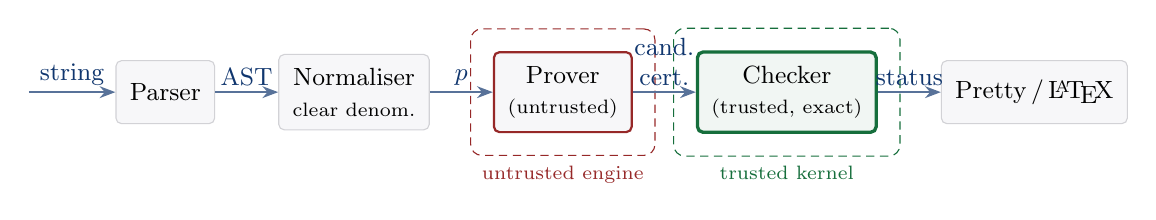
\begin{tikzpicture}[
  font=\small,
  node distance=6mm and 8mm,
  box/.style={draw=Rule, rounded corners=2pt, fill=CodeBg, align=center,
    inner sep=5pt, minimum height=8mm},
  untrusted/.style={box, draw=UntrustRed, thick},
  trusted/.style={box, draw=TrustGreen, very thick, fill=TrustGreen!6},
  data/.style={align=center, inner sep=2pt, text=NavyBlue},
  arr/.style={-{Stealth[length=2mm]}, thick, draw=NavyBlue!70},
]
\node[box] (parse) {Parser};
\node[box, right=of parse] (norm) {Normaliser\\{\scriptsize clear denom.}};
\node[untrusted, right=of norm] (prov) {Prover\\{\scriptsize (untrusted)}};
\node[trusted, right=of prov] (chk) {Checker\\{\scriptsize (trusted, exact)}};
\node[box, right=of chk] (pretty) {Pretty\,/\,\LaTeX};

\draw[arr] ($(parse.west)+(-1.1,0)$) -- (parse.west)
  node[data, midway, above] {string};
\draw[arr] (parse) -- (norm) node[data, midway, above] {AST};
\draw[arr] (norm) -- (prov) node[data, midway, above] {$p$};
\draw[arr] (prov) -- (chk) node[data, midway, above] {cand.\\cert.};
\draw[arr] (chk) -- (pretty) node[data, midway, above] {status};

\begin{scope}[on background layer]
  \node[draw=UntrustRed, densely dashed, rounded corners, inner sep=8pt,
        fit=(prov), label={[text=UntrustRed,font=\scriptsize]below:untrusted engine}] {};
  \node[draw=TrustGreen, densely dashed, rounded corners, inner sep=8pt,
        fit=(chk), label={[text=TrustGreen,font=\scriptsize]below:trusted kernel}] {};
\end{scope}
\end{tikzpicture}
\caption{The A\,$\ge$\,B pipeline. Only the checker is trusted; a fault in the
prover can cause a missed proof, never a false one.}
\label{fig:pipeline}
\end{figure}

\subsection{Module layering}

The library is layered so that each module depends only on those below it, which
keeps the trusted checker's dependencies minimal:
\[
  \begin{aligned}
    \textsf{Rational} &\to \textsf{Monomial} \to \textsf{Polynomial}
      \to \{\textsf{Ast},\ \textsf{Pretty}\} \\
    &\to \{\textsf{Parser},\ \textsf{Normalizer},\ \textsf{Certificate},\
      \textsf{Constrained}\}
      \to \textsf{Checker} \to \textsf{Prover}.
  \end{aligned}
\]
\textsf{Rational} is the sole point of contact with the bignum backend, which
localises the exact-arithmetic dependency (and eases a future pure-rational or
formally verified reimplementation).

\subsection{Command-line surface}

The tool exposes \texttt{prove "<inequality>"} (parse, clear denominators, and
search---side conditions may be attached with \texttt{given}, e.g.\
\texttt{a*b >= 0 given a >= 0, b >= 0}); \texttt{check <cert.json>} (load and
verify a certificate, plain or constrained); and \texttt{lean "<inequality>"}
(prove, then emit a machine-checkable Lean proof, Section~\ref{sec:lean}). Every
run reports one of four statuses with matching exit codes: \textsc{Proved},
\textsc{No\_Cert\_Found}, \textsc{Invalid\_Input}, \textsc{Check\_Failed}.

% ===========================================================================
\section{Validation}
\label{sec:validation}
% ===========================================================================

The proofs above argue that the system is sound; a benchmark corpus is how I keep
myself honest that it is also \emph{useful}, and stays that way as the code
changes. It holds $119$ inequalities, each tagged with a category and the status
the system ought to return (Table~\ref{tab:corpus}), drawn from classical results
(AM--GM, Cauchy--Schwarz, Schur), named competition problems (IMO, APMO, and
several national olympiads), and a standard olympiad reference---together with a
handful of deliberate soundness traps.

\begin{table}[h]
\centering
\begin{tabular}{@{}llc@{}}
\toprule
Category & Meaning & Expected status \\
\midrule
\texttt{in\_scope\_sos} & nonnegative on $\R^n$, SOS over $\Q$ & \textsc{Proved} \\
\texttt{out\_of\_scope\_v1} & true only under side constraints & \textsc{No\_Cert\_Found} \\
\texttt{not\_sos} & nonnegative but not SOS (Motzkin, Choi--Lam) & \textsc{No\_Cert\_Found} \\
\texttt{false} & deliberately false & \textsc{No\_Cert\_Found} \\
\bottomrule
\end{tabular}
\caption{Corpus categories and the status each should elicit.}
\label{tab:corpus}
\end{table}

Three independent harnesses guard the corpus: one runs every SOS certificate
through the trusted checker; one is an \emph{independent} numeric oracle that
random-samples each claim on its domain (implemented in a different language, so
an error in the core cannot mask a bad entry); and one enforces the
\emph{soundness gate}---no \texttt{false}, constrained, or \texttt{not\_sos}
entry may ever be proved. The gate is not decorative: it flagged a
problem originally recorded as requiring positivity, whose difference is in fact
the perfect square
\[
  (a+b)^2(a+c)^2 - 4abc(a+b+c) = (a^2 + ab + ac - bc)^2 ,
\]
prompting its reclassification as an unconditional SOS identity.

% ===========================================================================
\section{Formal verification in Lean 4}
\label{sec:lean}
% ===========================================================================

Proposition~\ref{prop:checker} is the hinge the entire design turns on, so it is
the one claim most worth putting beyond doubt. Two mechanisations in Lean~4, both
complete, now do that---from two different angles.

\subsection{A verified checker}

The first reimplements the checker over Mathlib's
\texttt{MvPolynomial (Fin\,$n$)\,$\Q$} and proves its soundness as a theorem the
Lean kernel checks:
\[
  \texttt{checkSOS}\ p\ \mathit{cert} = \texttt{true}
  \;\Longrightarrow\;
  \forall\,\x : \mathrm{Fin}\,n \to \R,\ \ 0 \le \operatorname{aeval} \x\, p .
\]
This is Proposition~\ref{prop:checker}, word for word, and its proof is the
formal shadow of Theorem~\ref{thm:soundness}: once \texttt{checkSOS} has forced
the identity $p = \sum_i c_i q_i^2$, nonnegativity falls straight out of
\texttt{sq\_nonneg}, \texttt{mul\_nonneg}, and \texttt{List.sum\_nonneg}. The
proof is complete and axiom-clean---\texttt{\#print axioms} reports only the
three standard Mathlib axioms (\texttt{propext}, \texttt{Classical.choice},
\texttt{Quot.sound}) and not a single \texttt{sorry}. And because Lean~4 compiles
to native code, this is not merely a proof \emph{about} a checker; it is a
checker that runs, and could stand as an independent oracle beside the OCaml one.

\subsection{One machine-checked proof per inequality}

The second goes further and makes each individual \emph{proof} machine-checked.
The command \texttt{a-geq-b lean "<inequality>"} runs the search, re-checks the
certificate, and emits a self-contained Lean file: a theorem $0 \le p$ over real
variables whose proof rewrites $p$ into its sum-of-squares form with
\texttt{ring}---the identity the checker has already verified---and then closes
it with \texttt{positivity}. Feeding that file to Lean has its kernel certify the
result, so an $A \ge B$ proof becomes a theorem in a general-purpose proof
assistant. It is untrusted output in the best possible sense: a bogus certificate
can only ever produce a Lean file that fails to compile, never a false theorem.

% ===========================================================================
\section{Roadmap}
\label{sec:roadmap}
% ===========================================================================

Much of the design is in place: the trusted checker and its Lean-verified twin
(Section~\ref{sec:lean}), the exact SOS prover, denominator clearing, and the
constrained search of Section~\ref{sec:constrained}. What is left sharpens the
prover, and---as always---keeps the checker the sole authority.

\smallskip
\noindent\textbf{A wide semidefinite prover.} The single remaining lever. Build
the monomial basis by the Newton-polytope reduction \eqref{eq:newton-basis} and
replace the bounded grid search with a genuine SDP over the affine family
\eqref{eq:match}: the exact core emits the Gram program, a numerical solver (an
interior-point method) returns an approximate PSD $Q$, and the core recovers an
exact certificate by \emph{Peyrl--Parrilo rounding}---projecting the numerical
Gram onto the affine subspace \eqref{eq:match}, which stays rational and remains
PSD when the numerical solution is strictly interior---before re-verifying. The
numerical code is thereby quarantined cleanly behind the trust boundary. The
constrained search of Section~\ref{sec:constrained} wants the very same machinery
for its hardest cases: a non-constant square multiplier $\sigma_i$ on an
inequality is itself a Gram problem, and so is a product of three or more
hypotheses.

\smallskip
\noindent The interface is deliberately the command line: \texttt{prove},
\texttt{check}, and \texttt{lean} print a structured, aligned report.

With the verified checker already in hand, finishing the wide prover would
realise a principled three-language architecture: exact symbolic computation and
the trusted core in a typed functional language (OCaml), numerical semidefinite
programming---untrusted---in the scientific-computing ecosystem (Python), and a
machine-checked proof of the kernel in a proof assistant (Lean~4). Each language
does what it is best at, and only the smallest of them has to be believed.

% ===========================================================================
\section*{References (selected)}
\addcontentsline{toc}{section}{References (selected)}
% ===========================================================================
\begin{enumerate}[label={[\arabic*]},leftmargin=2.2em]
  \item D.~Hilbert. \emph{Über die Darstellung definiter Formen als Summe von
    Formenquadraten.} Math.\ Ann.\ \textbf{32} (1888), 342--350.
  \item T.~S.~Motzkin. \emph{The arithmetic-geometric inequality.} In
    \emph{Inequalities} (1967), 205--224.
  \item M.~D.~Choi, T.~Y.~Lam. \emph{Extremal positive semidefinite forms.}
    Math.\ Ann.\ \textbf{231} (1977), 1--18.
  \item B.~Reznick. \emph{Extremal PSD forms with few terms.} Duke Math.\ J.\
    \textbf{45} (1978), 363--374.
  \item V.~Powers, T.~Wörmann. \emph{An algorithm for sums of squares of real
    polynomials.} J.\ Pure Appl.\ Algebra \textbf{127} (1998), 99--104.
  \item P.~A.~Parrilo. \emph{Semidefinite programming relaxations for
    semialgebraic problems.} Math.\ Program.\ \textbf{96} (2003), 293--320.
  \item H.~Peyrl, P.~A.~Parrilo. \emph{Computing sum of squares decompositions
    with rational coefficients.} Theoret.\ Comput.\ Sci.\ \textbf{409} (2008),
    269--281.
  \item J.~B.~Lasserre. \emph{Global optimization with polynomials and the
    problem of moments.} SIAM J.\ Optim.\ \textbf{11} (2001), 796--817.
  \item R.~B.~Manfrino, J.~A.~G.~Ortega, R.~V.~Delgado. \emph{Inequalities: A
    Mathematical Olympiad Approach.} Birkhäuser, 2009.
\end{enumerate}

\end{document}
